\chapter{ANALYSE ET CONCEPTION}

\section{ANALYSE}
Une fois les besoins des utilisateurs connu, nous pouvons commencer à concevoir les volets de notre data warehouse. Pour cela, nous avons eu recours à la modélisation dimensionnelle qui est souvent associé aux entrepôts de données compte tenu de ses avantages.
Cependant, avant de se lancer dans la modélisation il est intéressant de classer les sujets récence selon la pertinence pour l’entreprise et la facilité de réalisation. Ce classement nous aidera à choisir l’activité à modéliser en premier lieu de manière à garantir des résultats satisfaisants pour l’entreprise.\\

\subsection{PROCESSUS DE MODÉLISATION}
 
 La conception d’un modèle dimensionnel passe par cinq étapes essentielles :
 \begin{list}{•}{ }
    \item Choix de l’activité a modéliser : ce choix se fait après classement des activités dans une matrice dite d’analyse des priorités [Kimball, 2004]. Cette matrice permet de connaître quelle activité choisir en premier. Le classement des sujets recensés, qui s’est fait en collaboration avec les décideurs de l’entreprise est illustre dans la figure suivante.
    \begin{figure}[!htbp]
	\begin{center}
		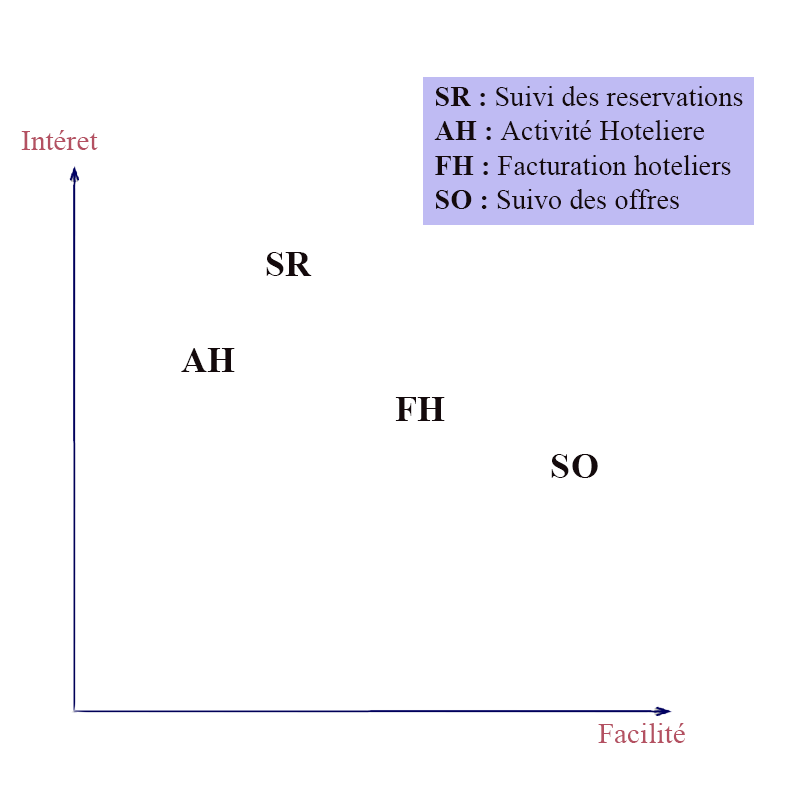
\includegraphics[scale=0.40]{images/priority.png}
		\caption{Analyse des priorités de Hosteline.}
		\label{use_bi_tools}
	\end{center}
	\end{figure}
    \item Définition de l’activité et de son grain
	\item Définition des dimensions qui décrivent une ligne de la table de fait
	\item Définir les mesurables du fait
    \item Définir les agrégats 
    
 \end{list}
 

\subsubsection{Volet « Réservation »}

\textbf{a)	Présentation de l’activité “Réservation”}\\
Selon Larousse, Une réservation est  \textit{l’action de retenir une place (dans un train, un avion, au théâtre, etc.), une table (au restaurant), une chambre (dans un hôtel)}.\\
La réservation sur Hosteline est au cœur de son activité réalisant la majorité de son chiffre d’affaire. Les chiffres lies à la réservation se présentent comme des indicateurs de grande signification par rapport a l’activité de l’entreprise. Ainsi la disponibilité de ces informations s’avère indispensable pour les décideurs de l’entreprise.\\

\textbf{b)	Grain de l’activité}\\
Le choix du grain le plus fin donne un maximum de flexibilité. Dans le cas des réservations le grain le plus fin, ou le niveau de détail le plus bas, correspond à une opération de réservation.

\textbf{c)	Dimensions participantes}\\
Les dimensions ont pour objectif de décrire un fait, Donc pour ce cas on essaye de recenser les informations qui décrivent au mieux une réservation.\\

\textbf{1 Dimension Temps}
La dimension temps est \textit{« la seul dimension qui figure systématiquement dans tout entrepôt de données, car en pratique tout entrepôt de données est une série temporelle. Le temps est le plus souvent la première dimension sou jacent de la base de données »} [Kimball, 2001]\\

La dimension temps se présente comme suit :

\begin{figure}[!htbp]
	\begin{center}
		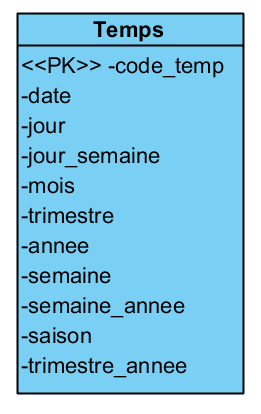
\includegraphics[scale=0.65]{images/dim_temps.png}
		\caption{Dimension temps du volet "Réservation".}
		\label{use_bi_tools}
	\end{center}
	\end{figure}

Le niveau de détail le plus bas de cette dimension est la journée. En effet, les utilisateurs ont fait ressortir le besoin de suivre les chiffres au jour le jour et d’en garder l'historique de ces derniers\\
Dans cette dimension, il est utilisé une clé artificielle comme clé primaire. Cette clé artificielle sert à faciliter la manipulation de la dimension.\\

\textbf{2 Dimension Client}\\
Le client s’impose comme un élément important dans l’analyse et intéresse les analystes et les décideurs de l’entreprise. Outre ce qu’il représente dans une opération de vente, l’analyse du comportement du client peut aider l’entreprise à mieux le satisfaire. La dimension client décrit un client, la personne qui réserve un hébergement.

\begin{figure}[!htbp]
	\begin{center}
		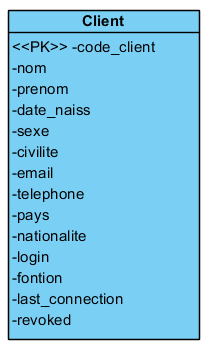
\includegraphics[scale=0.65]{images/dim_client.png}
		\caption{Dimension client du volet "Réservation".}
		\label{use_bi_tools}
	\end{center}
	\end{figure}

\textbf{3 Dimension Hôtel}
La réservation présentée plus haut est une convention entre un client et un hôtel. D’où le besoin d’une dimension hôtel. Cette dimension propose des axes d'analyses de grande importance déclinée dans la figure qui suit.
\cleardoublepage
\begin{figure}[!htbp]
	\begin{center}
		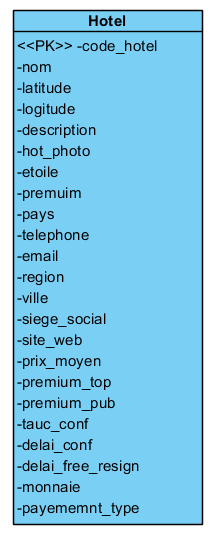
\includegraphics[scale=0.65]{images/dim_hotel.png}
		\caption{Dimension hotel du volet "Réservation".}
		\label{use_bi_tools}
	\end{center}
\end{figure}


\textbf{d) Les mesurables}\\
Les mesurables qui correspondent à l’activité des réservations et qui permettent de mesurer les performances de cette activité, sont la \textit{« Le CA des promotions \(CA\_res\_promo\) », « montant total des réservations \(CA\_reservation\) », «nombre de personne \(nbre\_personnes\)»}  et le \textit{« nombre de nuits \(nbre\_nuits\) »}.

\begin{figure}[!htbp]
	\begin{center}
		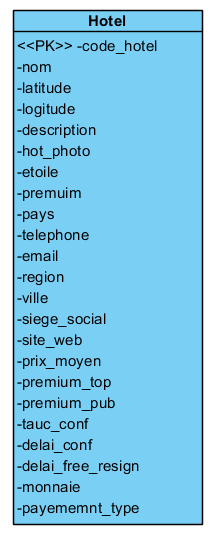
\includegraphics[scale=0.65]{images/dim_hotel.png}
		\caption{Table des faits du volet "Réservation".}
		\label{use_bi_tools}
	\end{center}
	\end{figure}

e) Le modèle en étoile de l’activité « Réservations »

\begin{figure}[!htbp]
	\begin{center}
		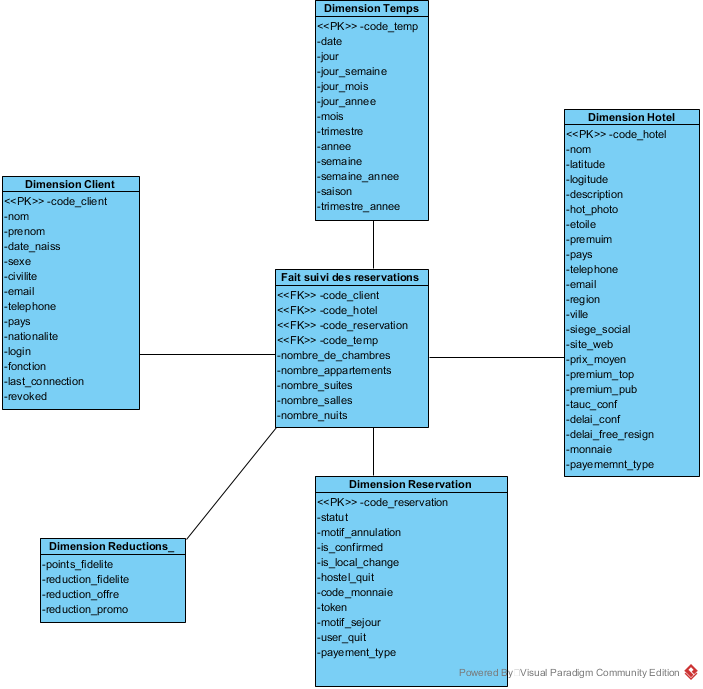
\includegraphics[scale=0.65]{images/star_reservations.png}
		\caption{Modèle en étoile du volet "Réservation".}
		\label{use_bi_tools}
	\end{center}
	\end{figure}

\textbf{f) Les agrégats}\\
Les tables d’agrégats améliorent les performances du Data Warehouse, en réduisant le nombre de lignes que le SGBD manipule afin de répondre à une requête. Cela se fait grâce à l’agrégation des données contenues dans les tables de faits détaillées et qui sont stockées dans de nouvelles tables de faits.
La construction des agrégats se base sur le modèle en étoile détaillée, et elle peut nécessiter:
\begin{list}{•}{ }
   \item La création de nouvelles dimensions dérivées : la construction d’un modèle agrégé nécessitera la suppression de quelques attributs d’une dimension qui désigne le grain le plus fin.
   \item La suppression de quelques dimensions : le modèle agrégé peut engendrer l’élimination de certaines dimensions qui n’apparaissent pas au niveau de détail voulu. On peut aussi :
   \item Créer de nouveaux faits: lors de la création de la table de faits agrégée on peut rajouter quelques faits qui n’existaient pas dans la modèle de base. En effet, l’usage et la signification des tables agrégées peuvent différer du modèle de base.
   \item  Créer des tables pré-jointes : une table d’agrégat peut être construite à partir d’une jointure entre la table de faits et une ou plusieurs dimensions. Le résultat est stocké dans une seule table dite pré-jointure. Une table d’agrégat peut être invisible ou visible à l’utilisateur final :
 \begin{list}{-}{ }
       \item Elle est invisible lorsqu’elle reflète exactement le modèle de base
       \item Elle est visible lorsqu’elle contient des faits supplémentaires.
 \end{list}
Les résultats issus d’une table agrégée ou du modèle de base doivent être identique.
Pour cette phase, on s’inspire de la démarche décrite par C. Adamson dans son livre
« Mastering the Data Warehouse Aggregates, Solution for Star Schema Performance ». La démarche consiste à :
\begin{enumerate}
 \item Enumérer les agrégats potentiels à partir d’une étoile détaillée : pour détecter les agrégats potentiels et choisir ceux à implémenter dans le Data Warehouse. Il est nécessaire de bien décrire chaque agrégat.
  \item Détecter les agrégats utiles : choisir des agrégats utiles à partir des agrégats potentiels.
  \item Construire le modèle agrégé : enfin on construit le modèle agrégé tout en prenant en considération les dimensions dérivées commune entre les différents modèles.
\end{enumerate}
\end{list}

\textbf{1- Les agrégats potentiels}

\begin{figure}[!htbp]
	\begin{center}
		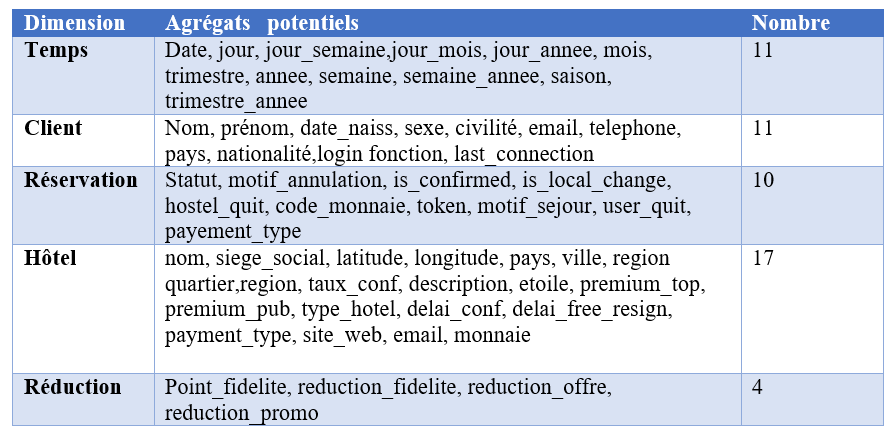
\includegraphics[scale=0.65]{images/tab_agregat_pot_reservation.png}
		\caption{Les agrégats potentiels du volet "Réservation".}
		\label{use_bi_tools}
	\end{center}
	\end{figure}
\cleardoublepage
\textbf{2	Les agrégats utiles}
\begin{figure}[!htbp]
	\begin{center}
		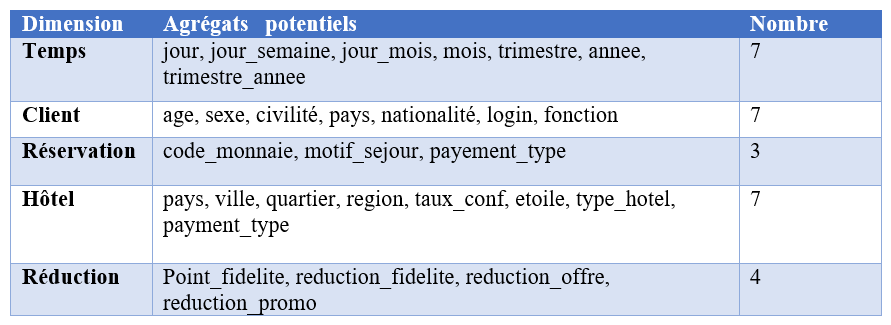
\includegraphics[scale=0.65]{images/tab_agregat_uti_reservation.png}
		\caption{Les agrégats utiles du volet "Réservation".}
		\label{use_bi_tools}
	\end{center}
	\end{figure}

A partir du tableau précédent nous choisissons les agrégats qui nous semblent les plus pertinents et susceptibles de faire l’objet d’accès fréquents. Nous arrêtons la liste des modèles agrégats suivants :
\begin{list}{•}{ }
\item Réservations journalières selon le lieu de provenance du client
\item Réservations journalières par nombre d’étoiles de l’hôtel
\item Taux de réservations par rapport aux réductions offertes.
\end{list}

 \subsubsection{Volet OFFRES}
\textbf{a)	Présentation des Offres}\\

Les offres constituent un des arguments marketing que possède la plateforme. Une offre est un pack constitué d’un ensemble d’hébergements et d’autres 

\textbf{b)	Grain de l’activité}\\
Le grain le plus fin de l’activité hôtelière correspond à : 
\begin{center}
\textit{Suivi des demandes faites à un hôtel à un endroit selon les réductions qu’il offre a une date donnée.}
\end{center}
\cleardoublepage
\textbf{f)	Les dimensions participantes du model}\\

Après la détection des dimensions de la nouvelle étoile, on procède à une mise en conformité des dimensions communes. Pour ce faire, on construit un tableau qui croise les étoiles conçues avec leurs dimensions. Le but étant de détecter les dimensions communes pour leurs mises en conformité. Le tableau suivant illustre cela.

\begin{figure}[!htbp]
	\begin{center}
		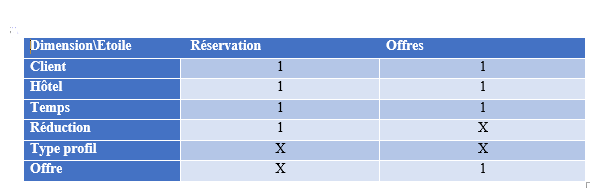
\includegraphics[scale=0.95]{images/tab_conform.png}
		\caption{Comparaison des volet Réservations et Offres.}
		\label{use_bi_tools}
	\end{center}
	\end{figure}

\textbf{Dimension Offre}\\]
 Cette dimension est primordiale pour une appréciation juste des indicateurs de ce modèle. Les axes d’étude qu’offre cette dimension sont mis en relief dans la figure qui suit. 

\begin{figure}[!htbp]
	\begin{center}
		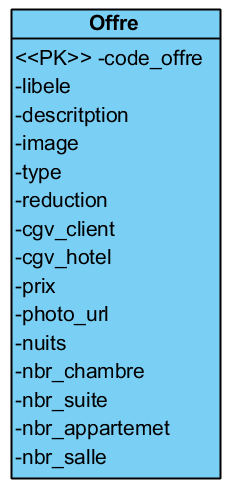
\includegraphics[scale=0.65]{images/dim_offre.png}
		\caption{Dimension offre du volet Offres.}
		\label{use_bi_tools}
	\end{center}
	\end{figure}
	
\cleardoublepage
\textbf{e) Le modèle en Etoile de l’activité « Suivi des Offres »}\\

\begin{figure}[!htbp]
	\begin{center}
		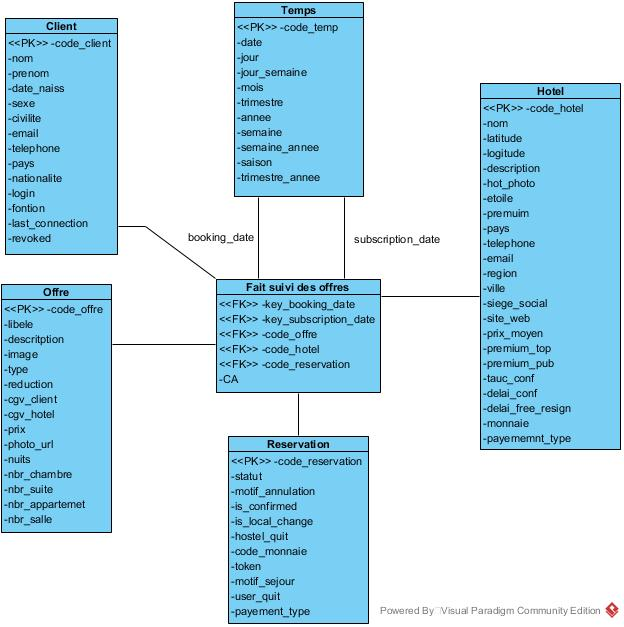
\includegraphics[scale=0.55]{images/star_offres.png}
		\caption{Modèle en étoile du volet "Offres".}
		\label{use_bi_tools}
	\end{center}
	\end{figure}


\textbf{1- Les agrégats potentiels}

\begin{figure}[!htbp]
	\begin{center}
		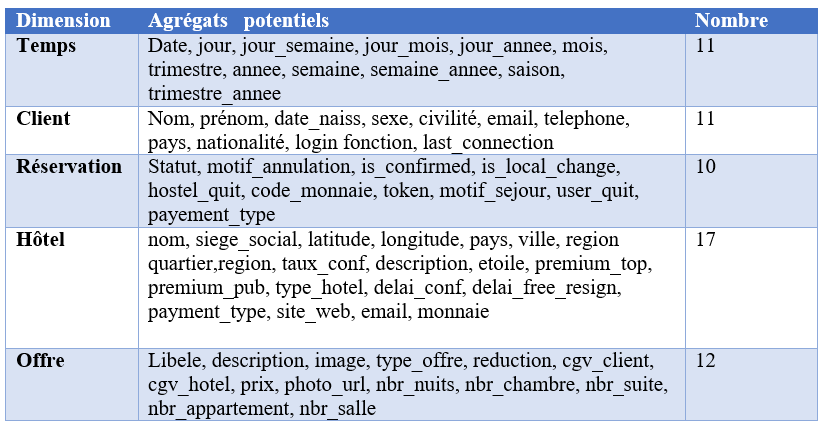
\includegraphics[scale=0.65]{images/tab_agregat_pot_offre.png}
		\caption{Les agrégats potentiels du volet "Offre".}
		\label{use_bi_tools}
	\end{center}
	\end{figure}
\cleardoublepage
\textbf{2	Les agrégats utiles}
\begin{figure}[!htbp]
	\begin{center}
		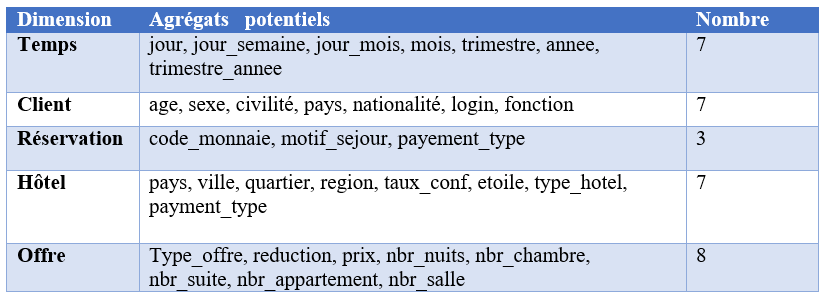
\includegraphics[scale=0.65]{images/tab_agregat_uti_offre.png}
		\caption{Les agrégats utiles du volet "Offre".}
		\label{use_bi_tools}
	\end{center}
	\end{figure}
	 
\section{CONCEPTION}


 


Afin de faciliter l'analyse et la navigation dans les données, il est important que les cubes dimensionnels soient bien conçues et définis de manière claire pour une utilisation intuitive.\\

    La conception des cubes dimensionnels passe par la définition des mesurables et des dimensions. Le but de la mise en place de ces cubes est d’offrir une représentation abstraite d'informations multidimensionnelles à des fins d’analyse. 


\subsection{Liste des cubes}
Dans ce qui suit nous allons dresser la liste des cubes à mettre en place. Pour chaque
cube on donnera les dimensions participantes ainsi que les mesurables présents dans ces
cubes.



	\begin{longtable}{|p{0.15\textwidth}|p{0.35\textwidth}|p{0.4\textwidth}|}
		\caption{Liste des cubes dimensionnels.} 
		\label{Liste des cubes dimensionnels}
		\\
		
		
		\hline 
		\textbf{Nom du cube} & 
		\textbf{Mesurables (Indicateurs)} &
		\textbf{Dimensions}
		\\
		
		
		\endfirsthead
		\caption[]{Liste des cubes dimensionnels (suite).} 
		\\
		\hline 
		\textbf{Nom du cube} & 
		\textbf{Mesurables (Indicateurs)} &
		\textbf{Dimensions}
		\\
		\hline
		\endhead
		\hline
		\endfoot
		\hline
		
		
		\hline
		Reservation &  
		
		\begin{description}
		 \item ca\_plateforme
		 \item ca\_hotel
		 \end{description} &
		 
		 \begin{description}
		 \item client
		 \item temps
		 \item type\_profile
		 \item reductions
		 \end{description}
		\\ 
		
		\hline
		Suivi des Offres &  
		\begin{description}
		 \item ca\_plateforme
		 \item nombre\_hotels
		 \item nombre\_reservations
		 \end{description} &
		\begin{description}
		 \item offre
		 \item temps
		 \item reservation
		 \item hotel
		 \item client
		 \end{description}
		\\
		
		\hline
		Suivi des hoteliers &  
		\begin{description}
		 \item ca\_reservation
		 \item ca\_reservation\_promo
		 \item nombre\_nuits
		 \item nombre\_nuitée
		 \item nombre\_chambre\_hotel
		 \end{description} &
		\begin{description}
		 \item temps
		 \item reservation
		 \item hotel
		 \item client
		 \item reductions
		 \end{description}
		\\  
		
		\hline
		facturation hotel &  
		\begin{description}
		 \item nombre\_hotels
		 \end{description} &
		\begin{description}
		 \item temps
		 \item reduction
		 \item hotel
		 \item client
		 \item type\_profile
		 \end{description}
		\\
		
		\hline
		Suivi des Offres &  
		\begin{description}
		 \item ca\_plateforme
		 \item nombre\_hotels
		 \item nombre\_reservations
		 \end{description} &
		\begin{description}
		 \item offre
		 \item temps
		 \item reservation
		 \item hotel
		 \item client
		 \end{description}
		\\
		
		\hline 
	\end{longtable} 

\cleardoublepage
\subsection{PRÉSENTATION DES DIMENSIONS}
\begin{figure}[!htbp]
	\begin{center}
		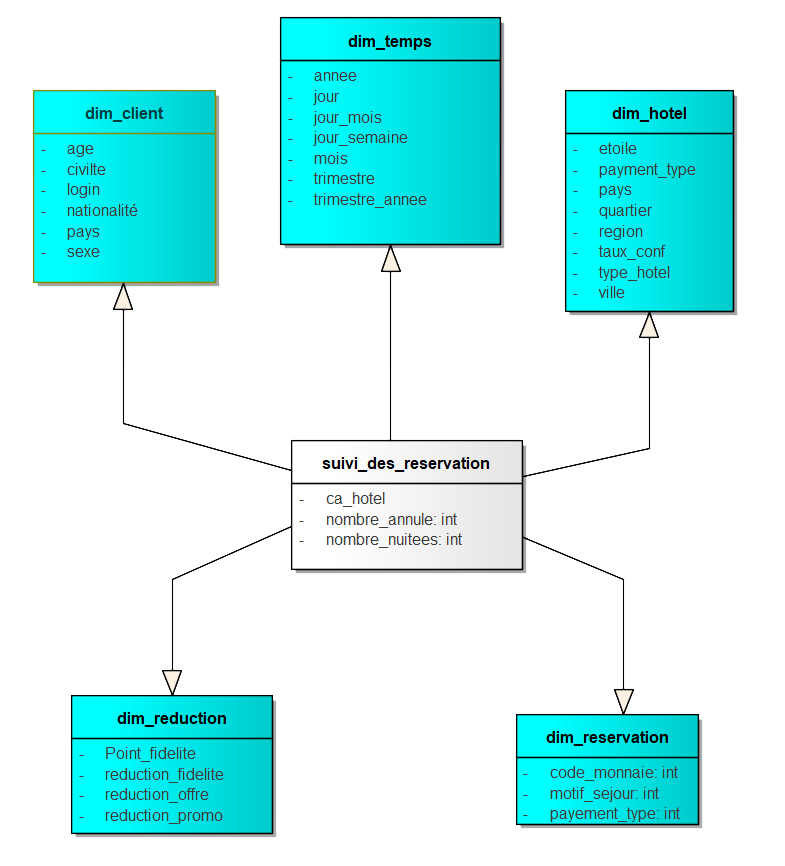
\includegraphics[scale=0.85]{images/cube_reservation.png}
		\caption{Cube dimensionnel « Suivi des reservations ».}
		\label{use_bi_tools}
	\end{center}
\end{figure}

\begin{figure}[!htbp]
	\begin{center}
		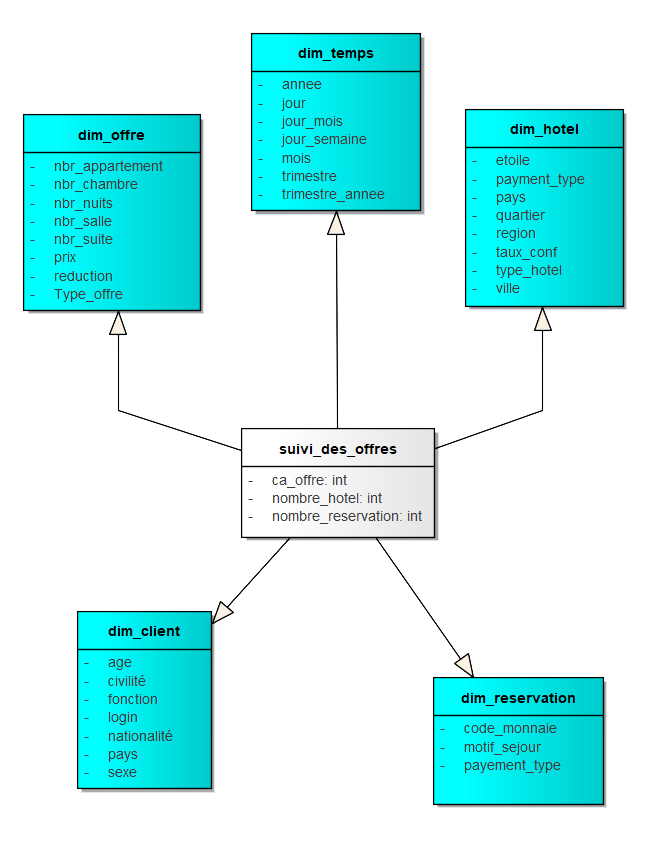
\includegraphics[scale=0.85]{images/cube_offre.png}
		\caption{Cube dimensionnel « Suivi de offres ».}
		\label{use_bi_tools}
	\end{center}
\end{figure}

\begin{figure}[!htbp]
	\begin{center}
		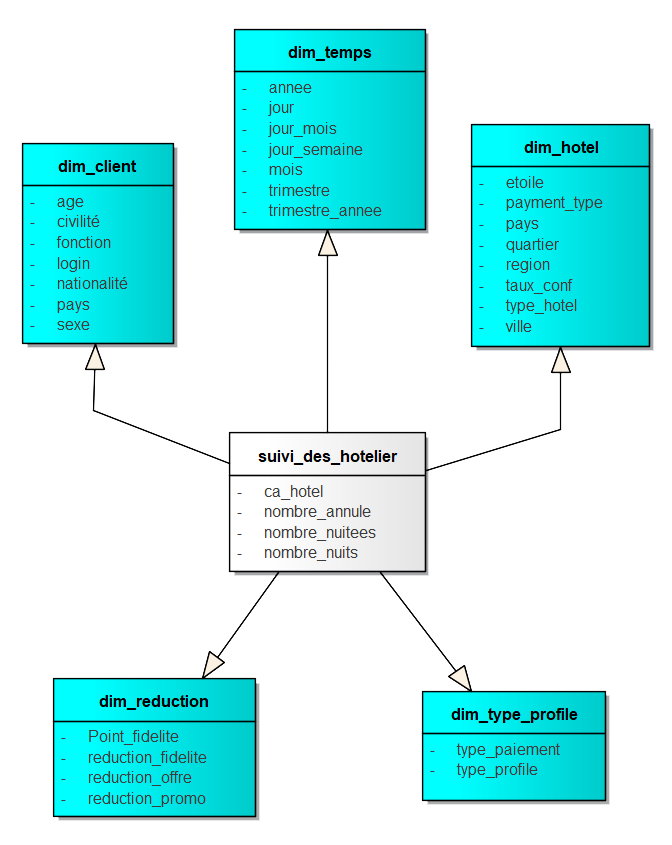
\includegraphics[scale=0.85]{images/cube_hotelier.png}
		\caption{Cube dimensionnel « Suivi des hoteliers ».}
		\label{use_bi_tools}
	\end{center}
\end{figure}

\begin{figure}[!htbp]
	\begin{center}
		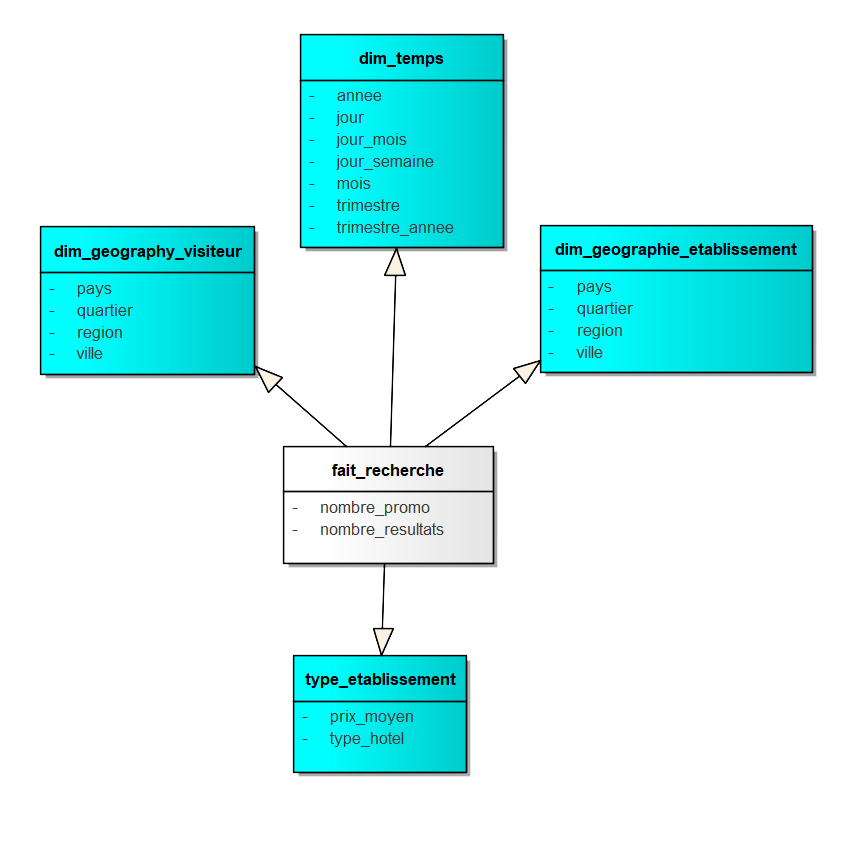
\includegraphics[scale=0.85]{images/cube_recherche.png}
		\caption{Cube dimensionnel « Recherche ».}
		\label{use_bi_tools}
	\end{center}
\end{figure}

